% Created: 2019-12-10
% Plot participant data
% http://github.com/zhaobn/magic_stones

\documentclass{article}
\title{[Magic Stones] Plots for Experiment 1}
\author{Bonan Zhao (b.zhao@ed.ac.uk)}

% Text formats: margin, font, spacing
\usepackage[margin=0.8in]{geometry}
\usepackage{charter}
\renewcommand{\baselinestretch}{1.3}

% Graphics
\usepackage{graphicx}
\usepackage{subcaption}
\graphicspath{{../figs/}}


\begin{document}
\maketitle

% Raw participant data
\section{Participant data}
\subsection{Raw data}

\begin{figure}[h!]
	\centering
  \begin{subfigure}[t]{0.31\textwidth}
  	\centering
  	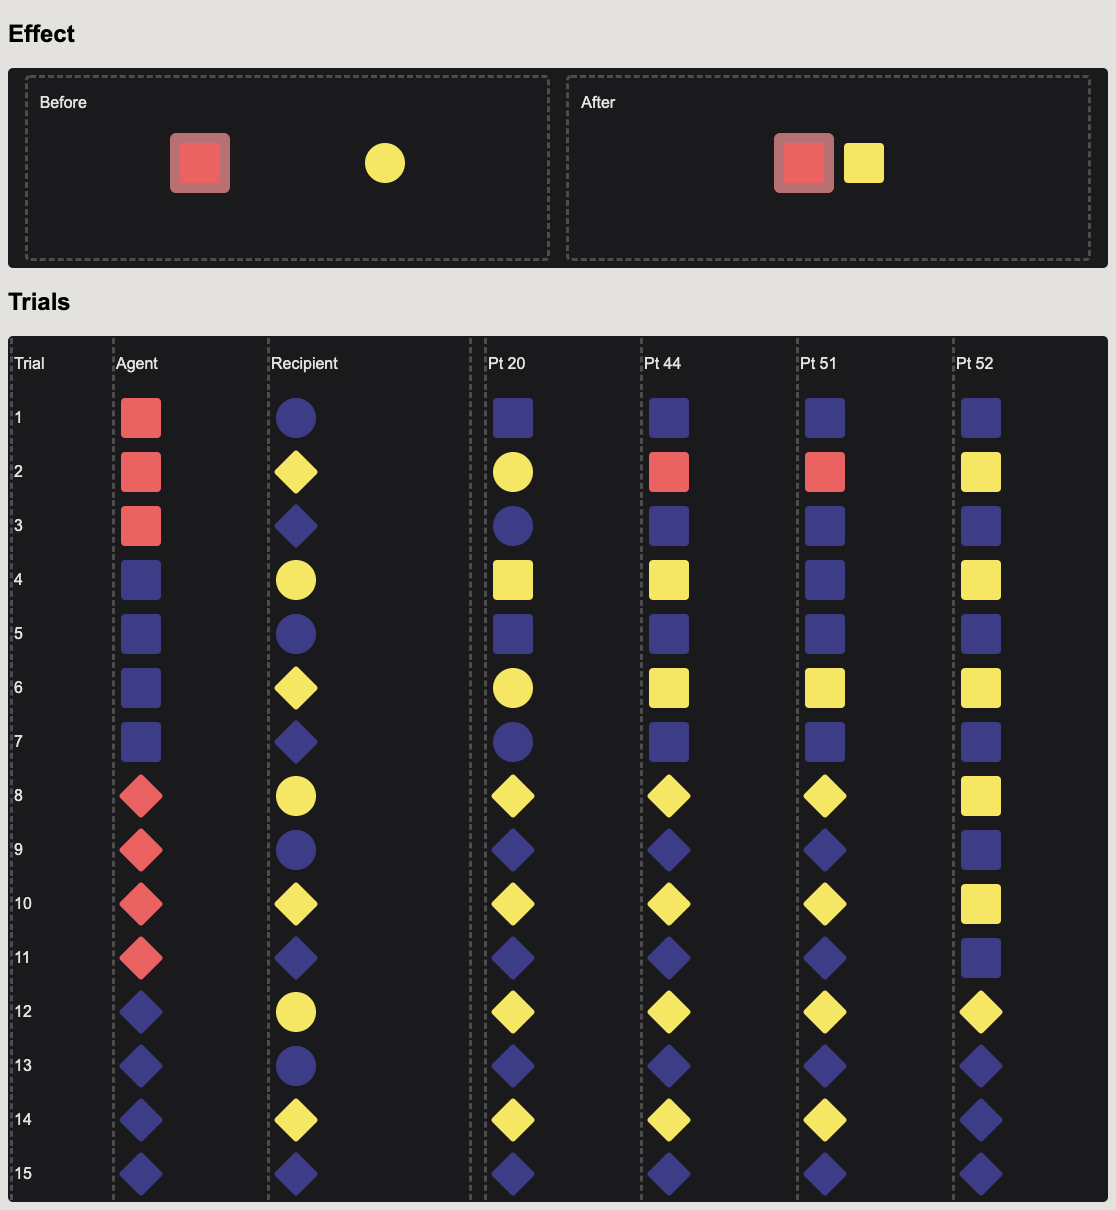
\includegraphics[width=\linewidth]{raw_g1} 
  	\caption{To the same shape} \label{fig:raw_g1}
  \end{subfigure}
  \hfill
  \begin{subfigure}[t]{0.31\textwidth}
  	\centering
  	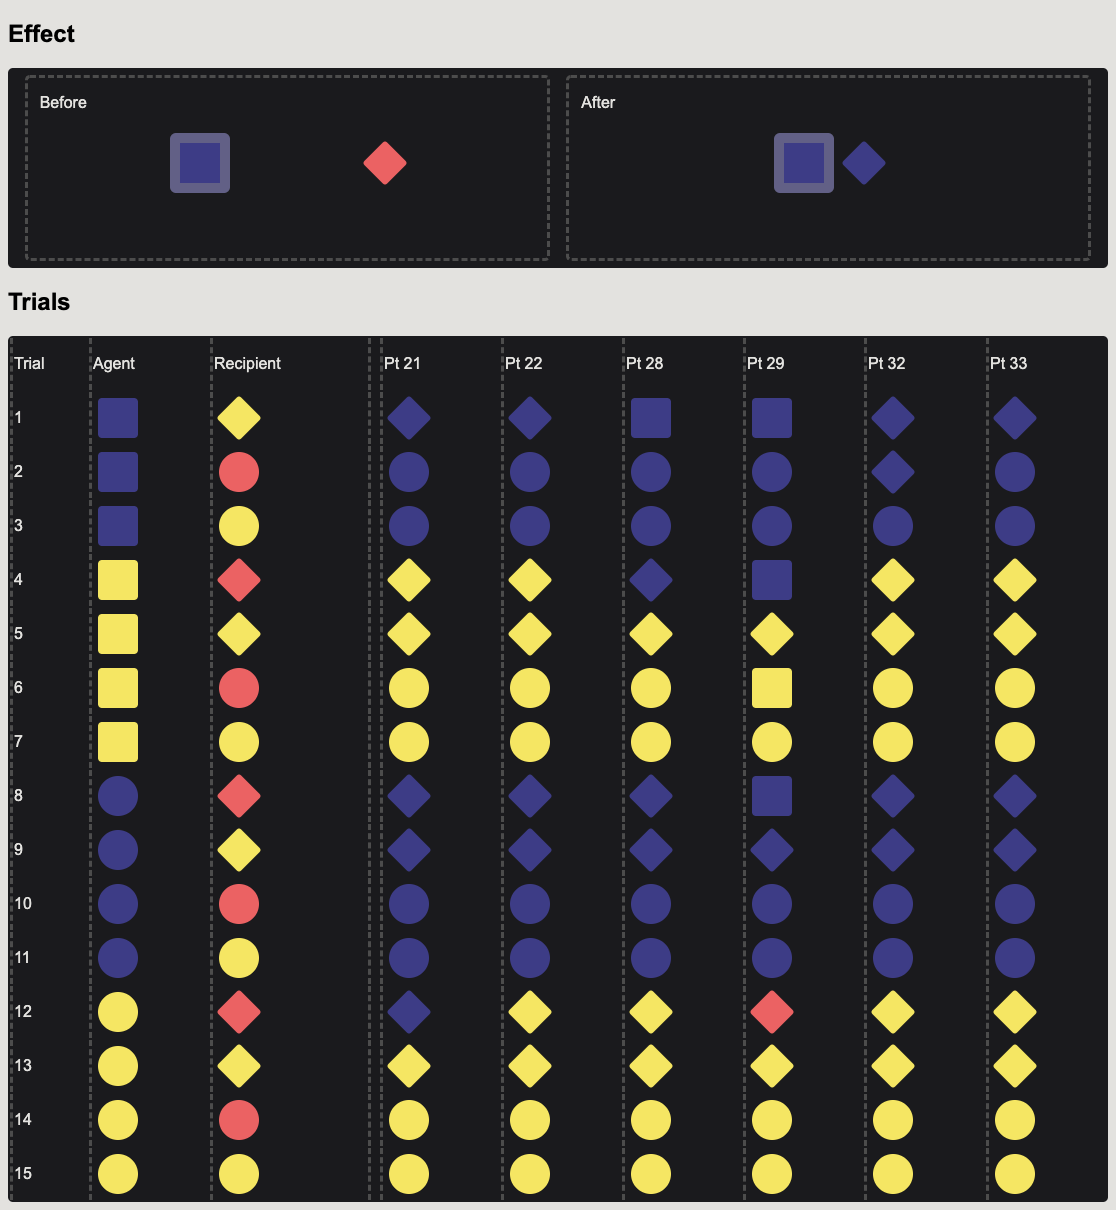
\includegraphics[width=\linewidth]{raw_g3} 
  	\caption{To the same color} \label{fig:raw_g3}
  \end{subfigure}
  \hfill
  \begin{subfigure}[t]{0.31\textwidth}
  	\centering
  	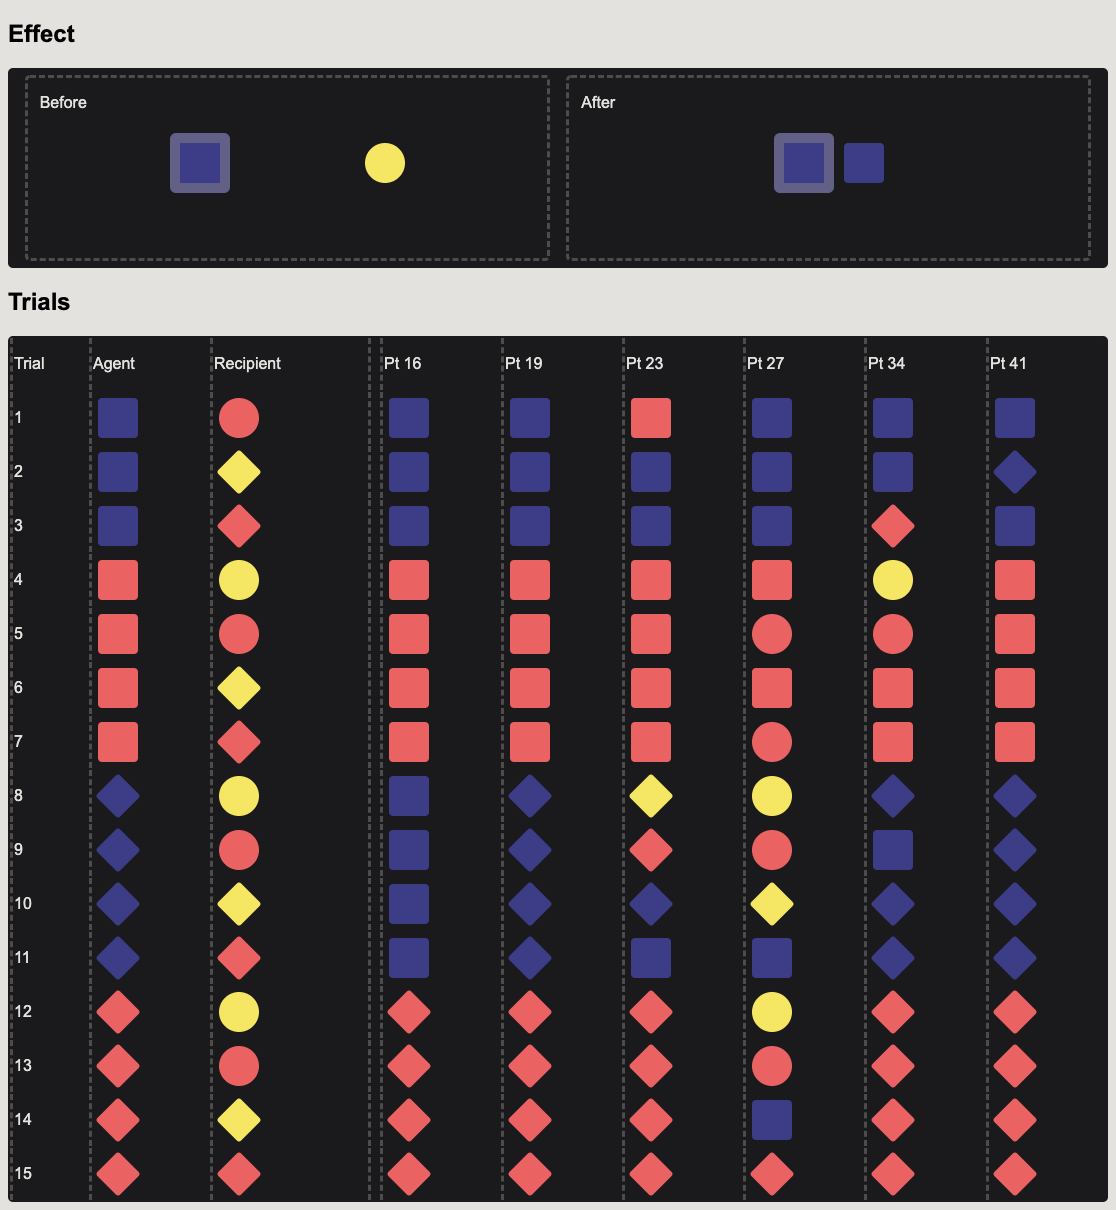
\includegraphics[width=\linewidth]{raw_g6} 
  	\caption{To the same object} \label{fig:raw_g6}
  \end{subfigure}

  \vspace{1em}
  \begin{subfigure}[t]{0.31\textwidth}
  	\centering
  	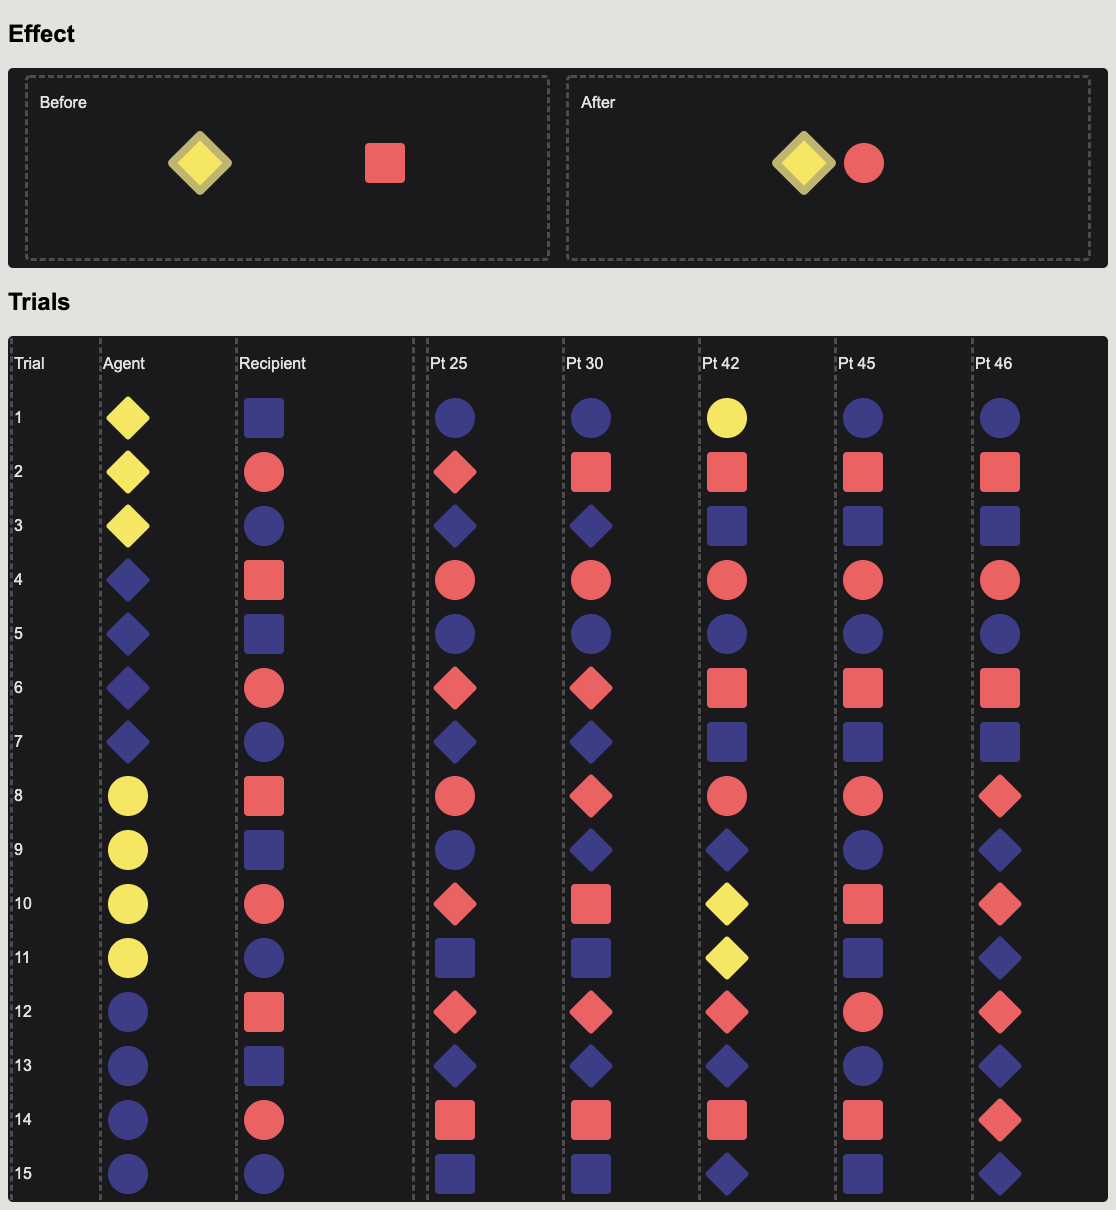
\includegraphics[width=\linewidth]{raw_g2} 
  	\caption{To a different shape} \label{fig:raw_g2}
  \end{subfigure}
  \hfill
  \begin{subfigure}[t]{0.31\textwidth}
  	\centering
  	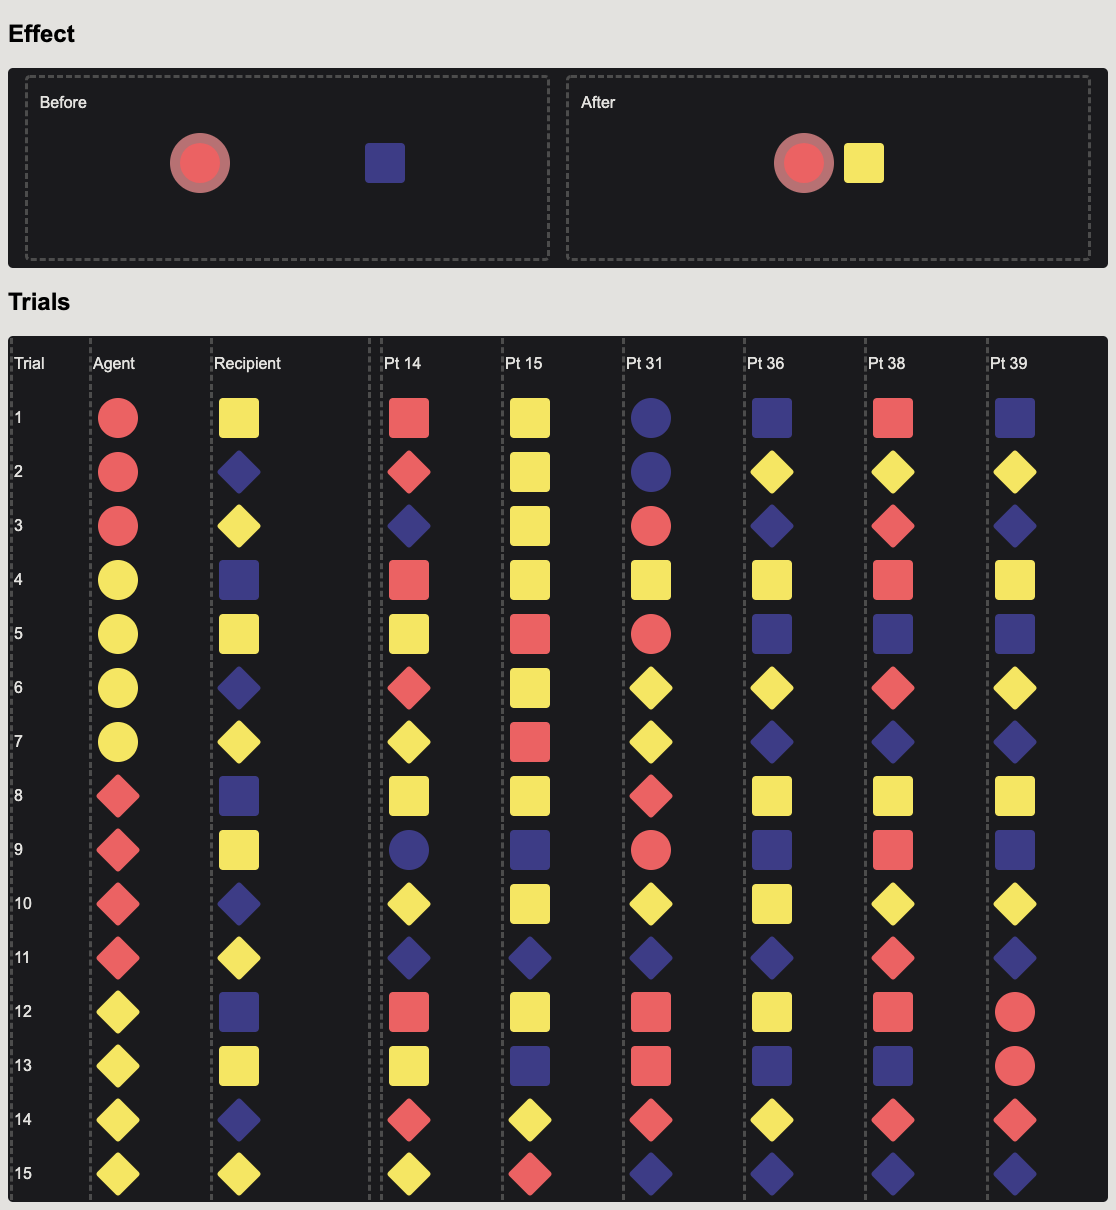
\includegraphics[width=\linewidth]{raw_g4} 
  	\caption{To a different color} \label{fig:raw_g4}
  \end{subfigure}
  \hfill
  \begin{subfigure}[t]{0.31\textwidth}
  	\centering
  	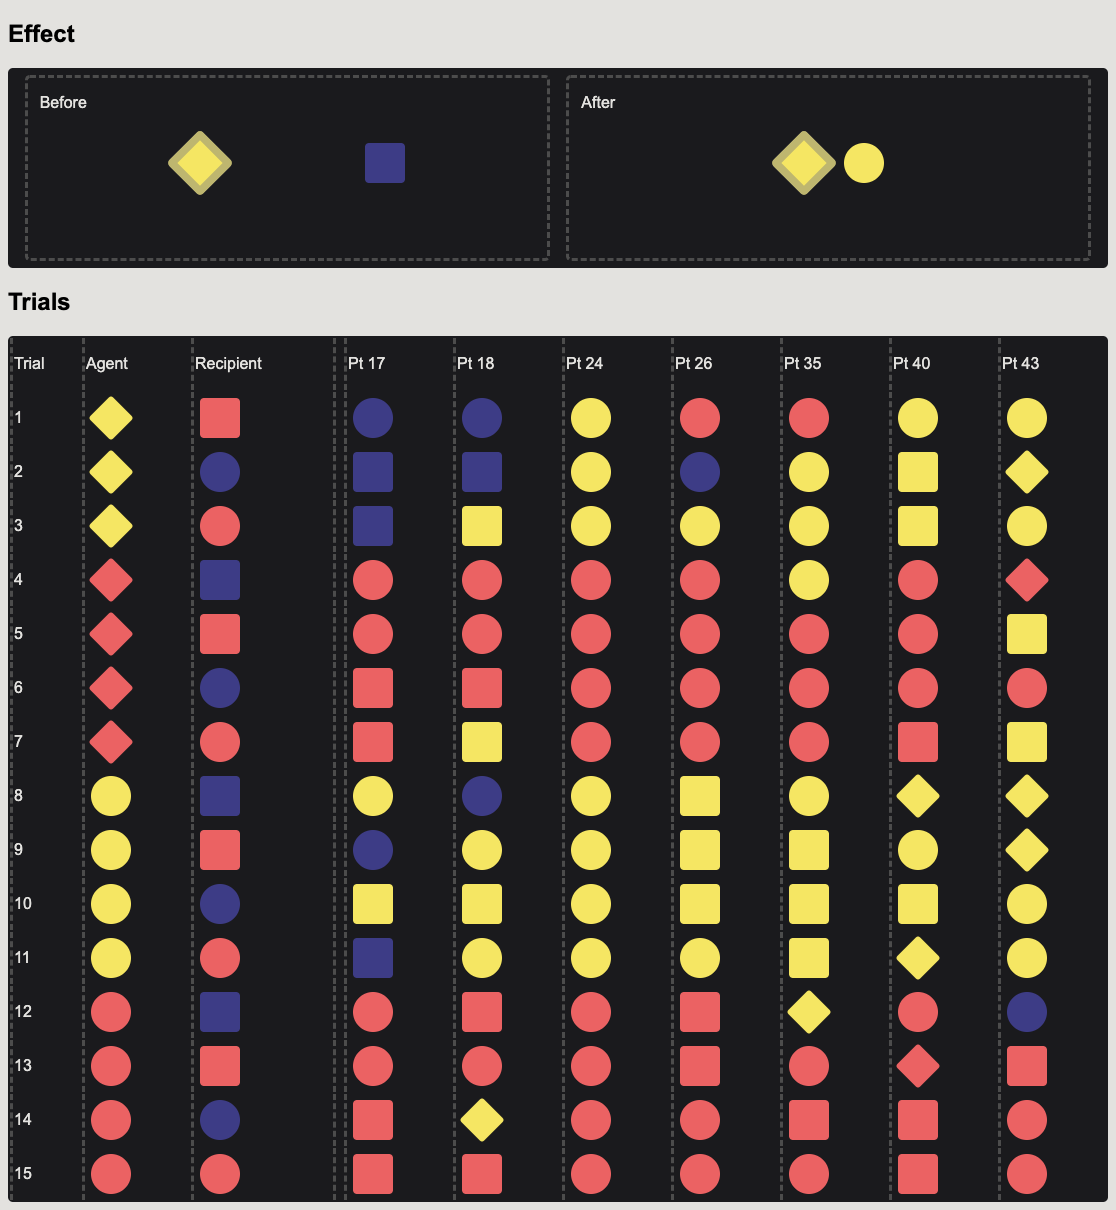
\includegraphics[width=\linewidth]{raw_g5} 
  	\caption{To a different object} \label{fig:raw_g5}
  \end{subfigure}
  \caption{Participant data per group per trial. Each figure is for one group - at the top is a summary of the magic effect participants watched, and below is a complete visualization of participant selections. In the selection part, each row is for one trial: the first two icons are the magic stone and normal stone that a participant is asked to make a prediction for, and the rest are participant selections.}
  % \caption{Some general caption of all the figures. In (\subref{fig:group01}) you can see a  green square....}
\end{figure}


\newpage
Obviously, generalizations are not random, as shown in Figure~\ref{fig:sum}. Take the third column from left for example, a dominant selection can be observed across 15 trials.

\begin{figure}[h!]
  \centering
  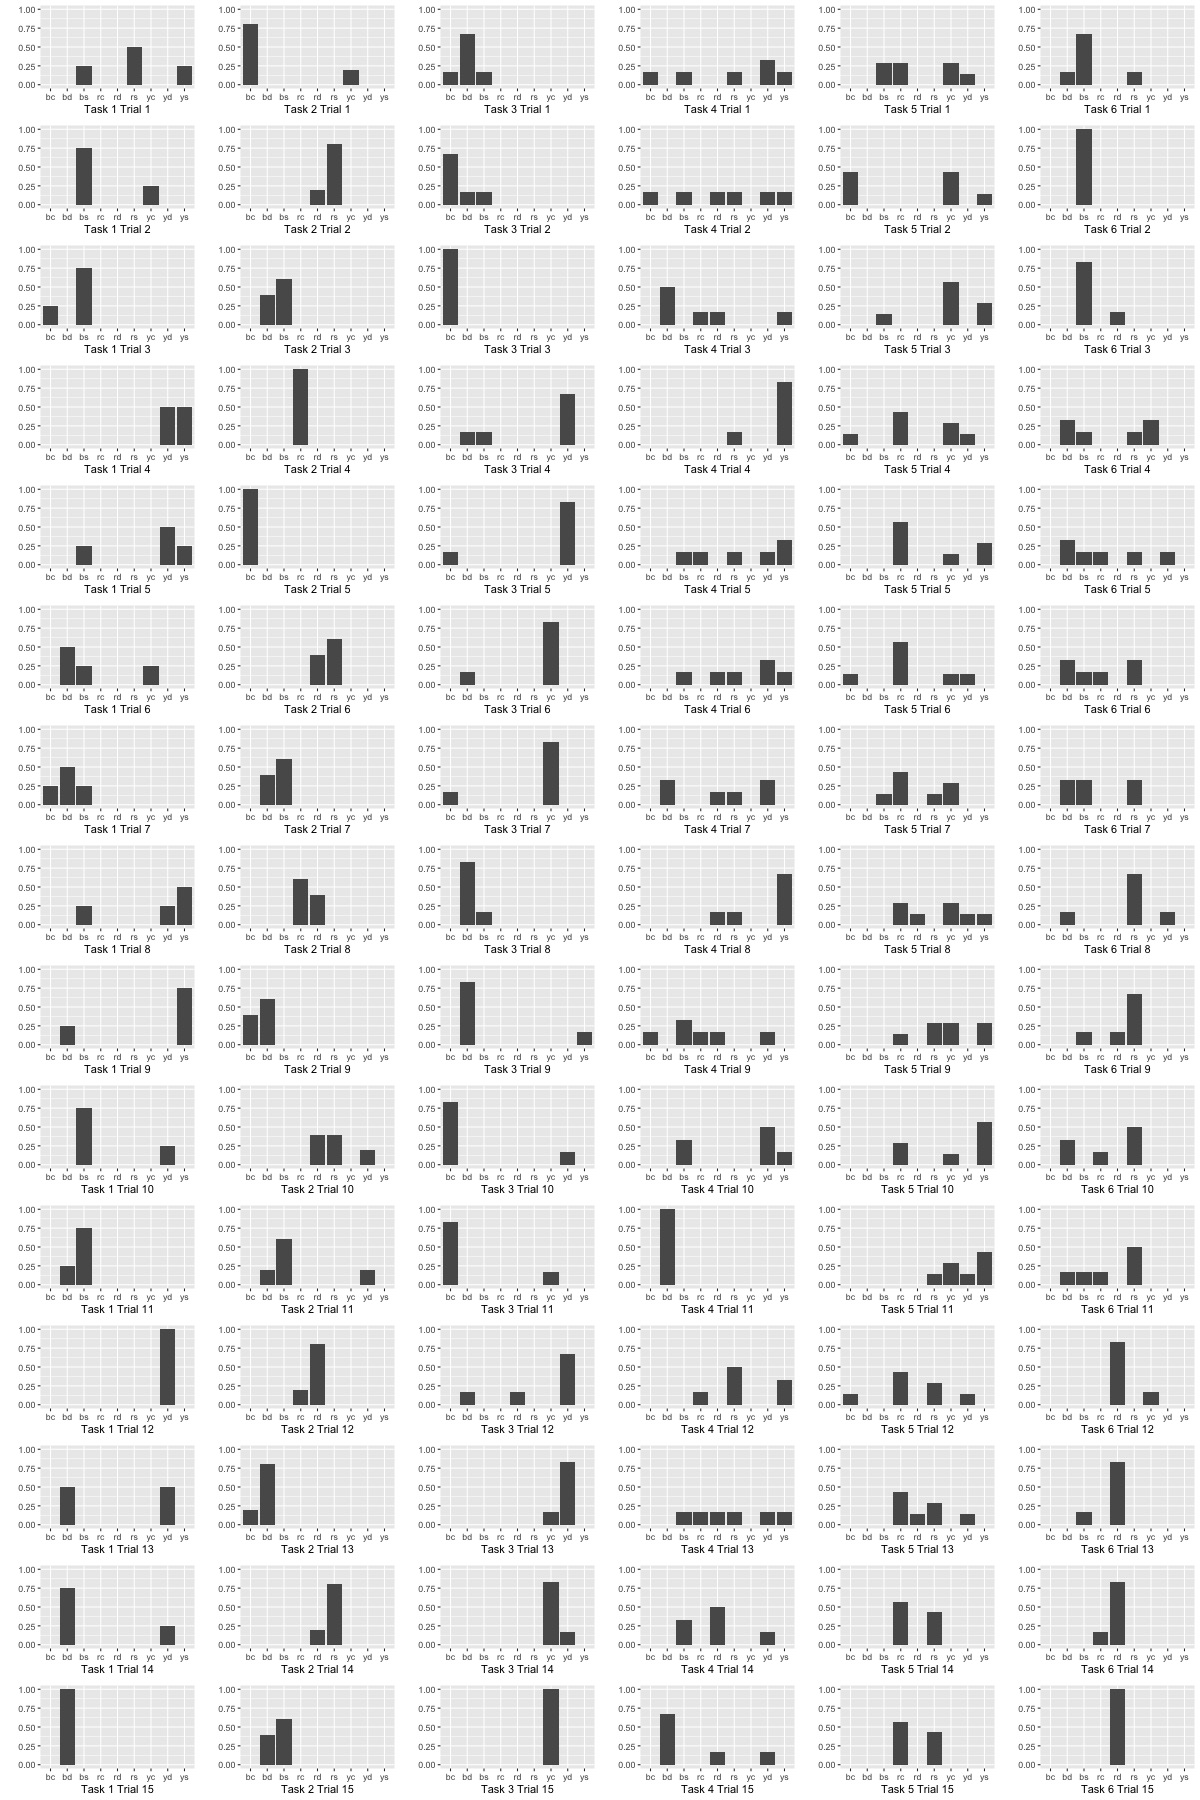
\includegraphics[width=.8\linewidth]{trials}
  \caption{Participant raw selections summary. Each row is for one trial, and each column is for one task. For each sub-figure, y-axis is percentage, and x-axis from left to right is: bc, bd, bs, rc, rd, rs, yc, yd, ys.}
  \label{fig:sum}
\end{figure}

\newpage
If we plot each participant selection relative to the agent stone and recipient stone in that generalization task, the uniformity of generalization is even clearer. In the last raw of Figure~\ref{fig:sum_rel}, almost everyone made a same choice across 6 different learning tasks. 

\begin{figure}[h!]
  \centering
  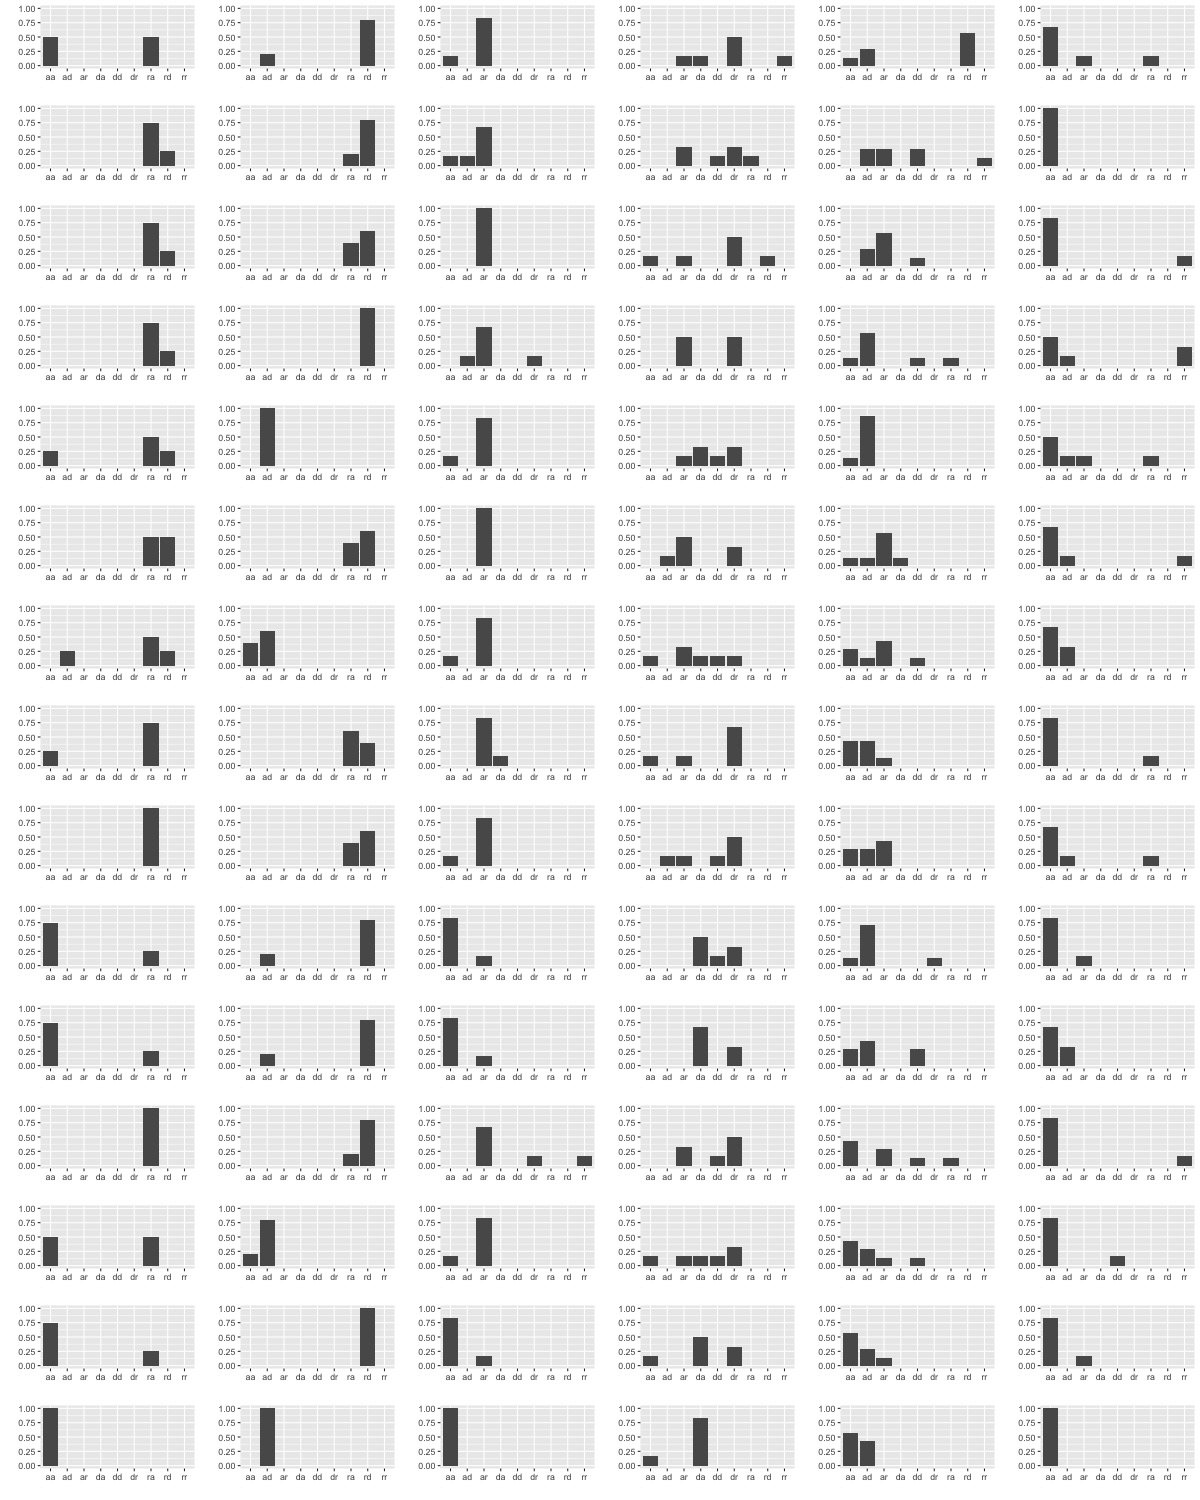
\includegraphics[width=.8\linewidth]{trials_relative}
  \caption{Relative selections summary. Each row is for one trial, and each column is for one task. For each sub-figure, y-axis is percentage, and x-axis from left to right is: aa, ad, ar, da, dd, dr, ra, rd, rr.}
  \label{fig:sum_rel}
\end{figure}

% Aggregated by groups
\newpage
\subsection{Aggregated by relative selection}

Between-subject aggregation shows that different learning tasks induce different generalization patterns, as illustrated by Figure~\ref{fig:agg_groups}.

\begin{figure}[h!]
  \centering
  \begin{subfigure}[t]{0.25\textwidth}
    \centering
    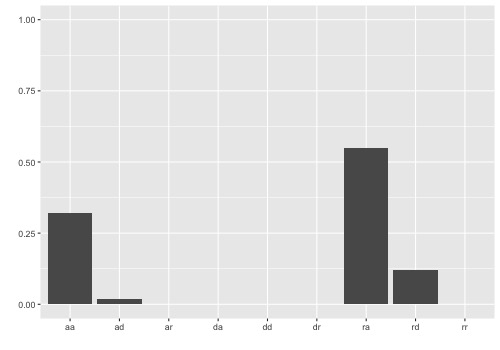
\includegraphics[width=\linewidth]{agg_g1} 
    \caption{To the same shape} \label{fig:agg_g1}
  \end{subfigure}
  \begin{subfigure}[t]{0.25\textwidth}
    \centering
    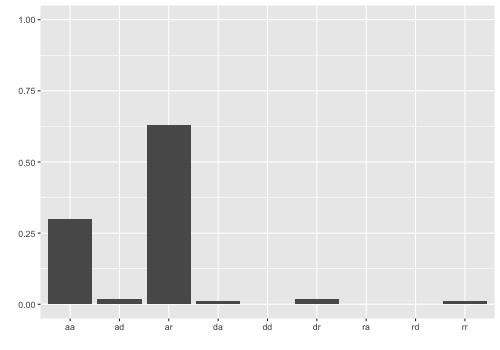
\includegraphics[width=\linewidth]{agg_g3} 
    \caption{To the same color} \label{fig:agg_g3}
  \end{subfigure}
  \begin{subfigure}[t]{0.25\textwidth}
    \centering
    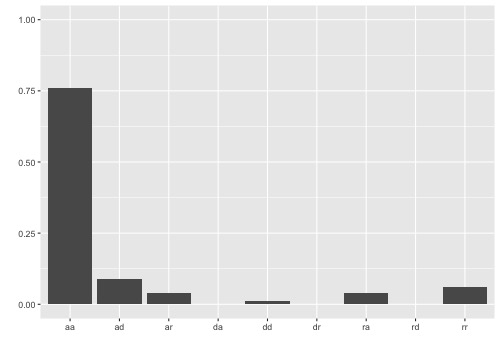
\includegraphics[width=\linewidth]{agg_g6} 
    \caption{To the same object} \label{fig:agg_g6}
  \end{subfigure}

  \vspace{1em}
  \begin{subfigure}[t]{0.25\textwidth}
    \centering
    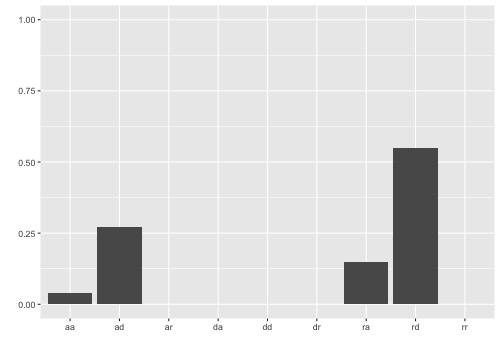
\includegraphics[width=\linewidth]{agg_g2} 
    \caption{To a different shape} \label{fig:agg_g2}
  \end{subfigure}
  \begin{subfigure}[t]{0.25\textwidth}
    \centering
    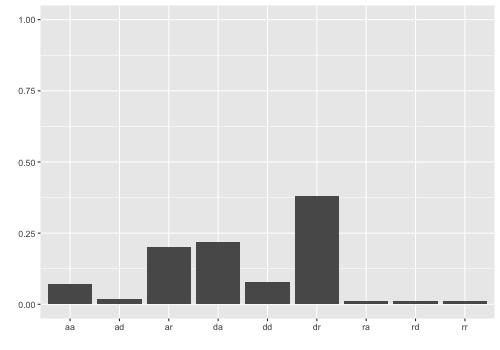
\includegraphics[width=\linewidth]{agg_g4} 
    \caption{To a different color} \label{fig:agg_g4}
  \end{subfigure}
  \begin{subfigure}[t]{0.25\textwidth}
    \centering
    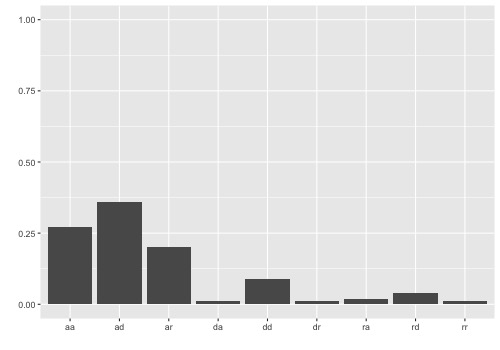
\includegraphics[width=\linewidth]{agg_g5} 
    \caption{To a different object} \label{fig:agg_g5}
  \end{subfigure}
  \caption{Aggregated relative selections per task. For each sub-figure, y-axis is percentage, and x-axis from left to right is: aa, ad, ar, da, dd, dr, ra, rd, rr.}
  \label{fig:agg_groups}
\end{figure}

% Aggregated by trials
Aggregation by trials (within-subject) emphasizes that while the generalization scenario further differs from the learning scenario, participants tend to make a more similar decision.

\begin{figure}[h!]
  \centering
  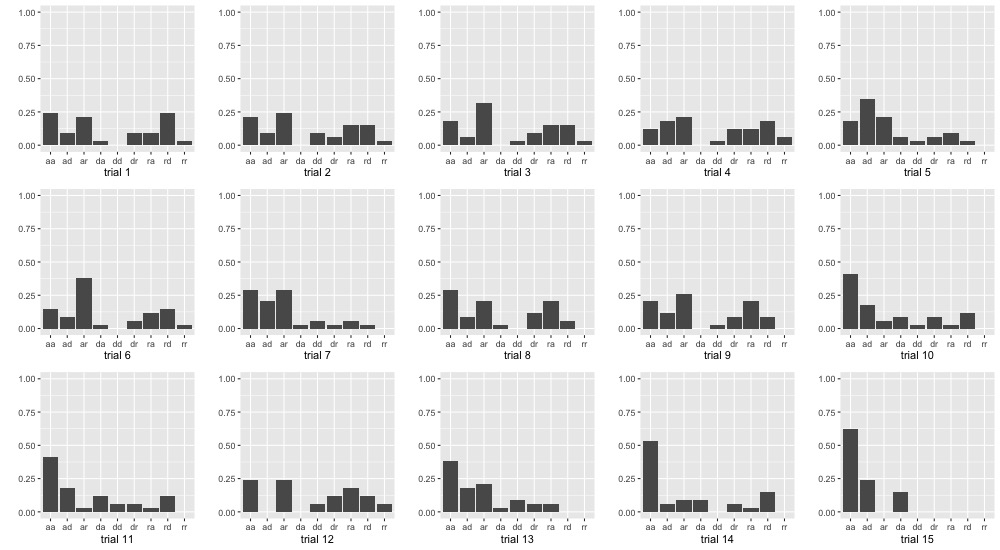
\includegraphics[width=.85\linewidth]{agg_trials}
  \caption{Aggregated relative selections per trial. For each sub-figure, y-axis is percentage, and x-axis from left to right is: aa, ad, ar, da, dd, dr, ra, rd, rr.}
\end{figure}

% Order effects
\newpage
\subsection{Order effects? Not really}

Comparing a randomized sequence of trials and ordered sequence of trials shows no significant difference.

\begin{figure}[h!]
  \centering
  \begin{subfigure}[t]{0.45\textwidth}
    \centering
    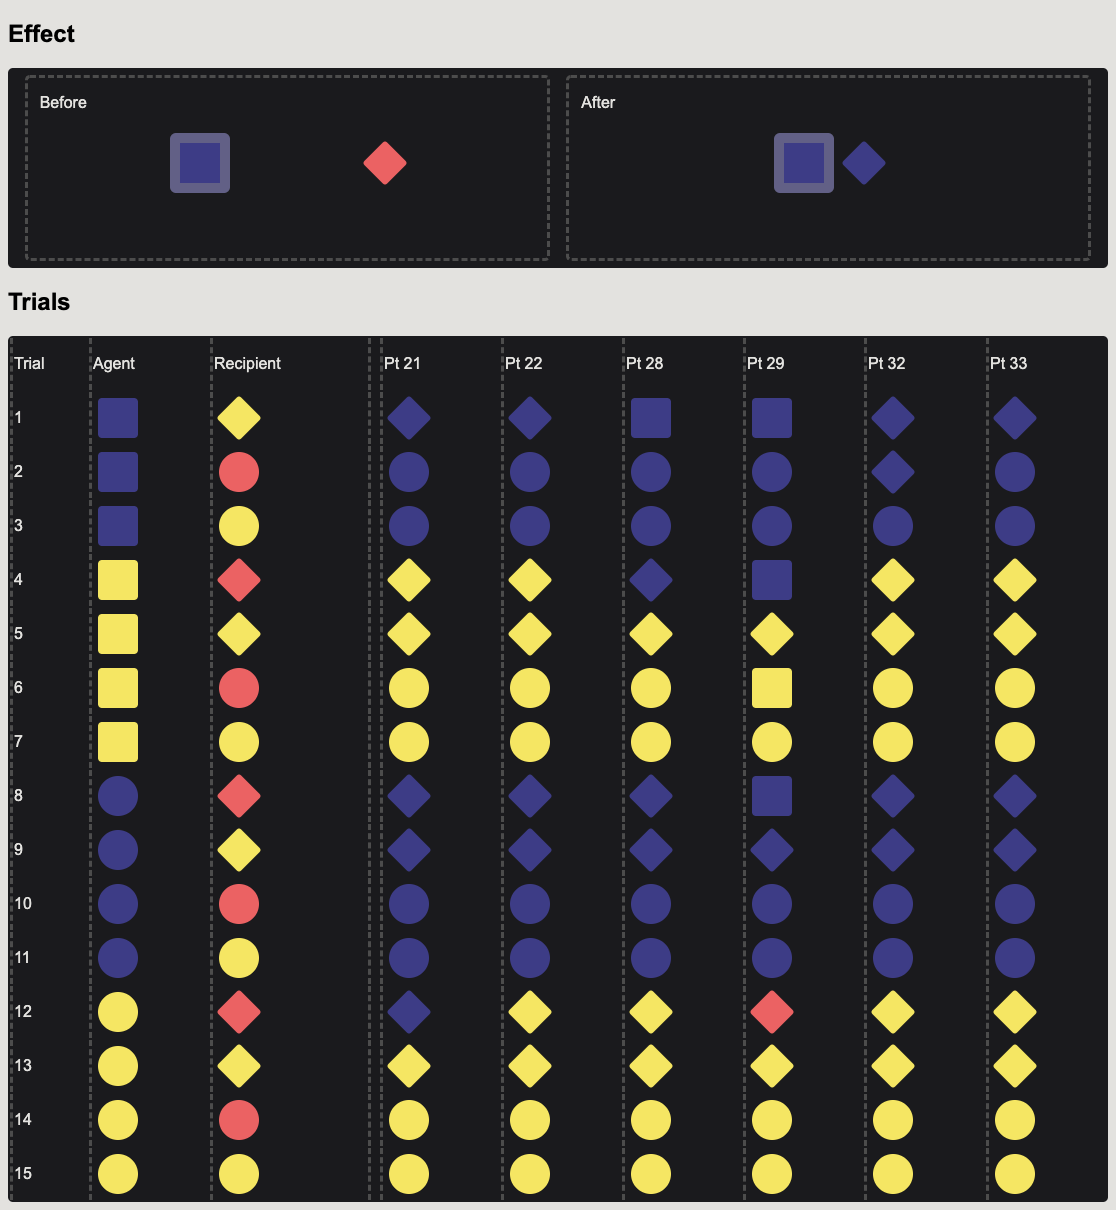
\includegraphics[width=\linewidth]{raw_g3} 
    \caption{Task 3 ordered.} \label{fig:raw_g3_ordered}
  \end{subfigure}
  \hfil
  \begin{subfigure}[t]{0.45\textwidth}
    \centering
    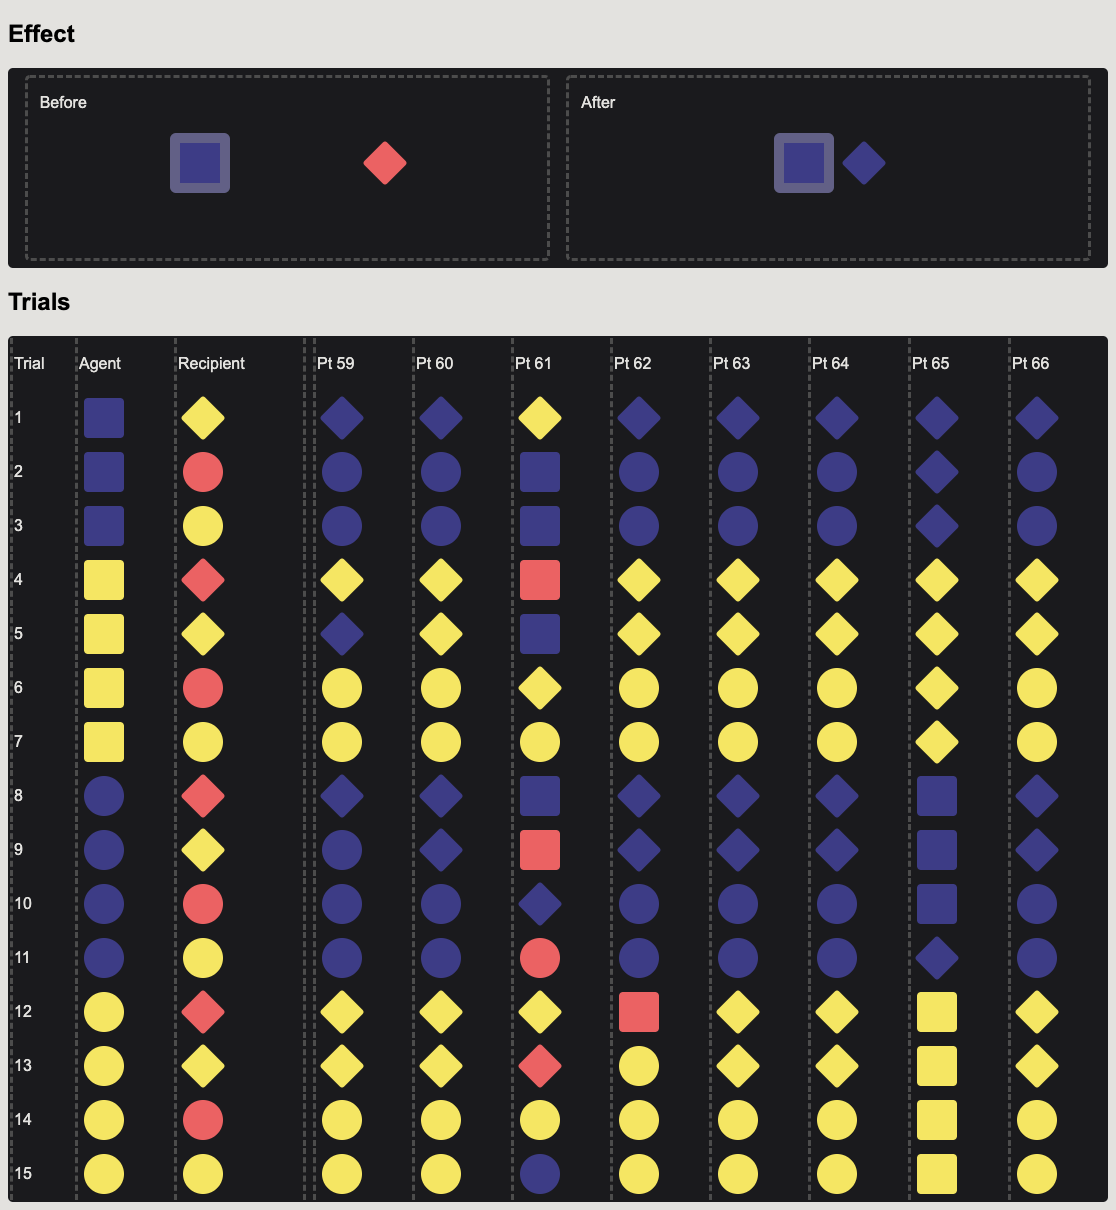
\includegraphics[width=\linewidth]{random} 
    \caption{Task 3 randomized.} \label{fig:random}
  \end{subfigure}
  \caption{Order does not effect generalization predictions.}
\end{figure}

% ----------------------------------------------
% ------------ Simulation data -----------------
% ----------------------------------------------

\newpage
\section{Normative model simulations}
\subsection{Raw simulations}

Different from the participant data, the normative model is more uncertain when the generalization scenario differs more from the learning task, as shown in the last few columns in Figure~\ref{fig:sim_raw}. In the same situation, humans tend to concentrate on one selection instead of choosing randomly.

\begin{figure}[h!]
  \centering
  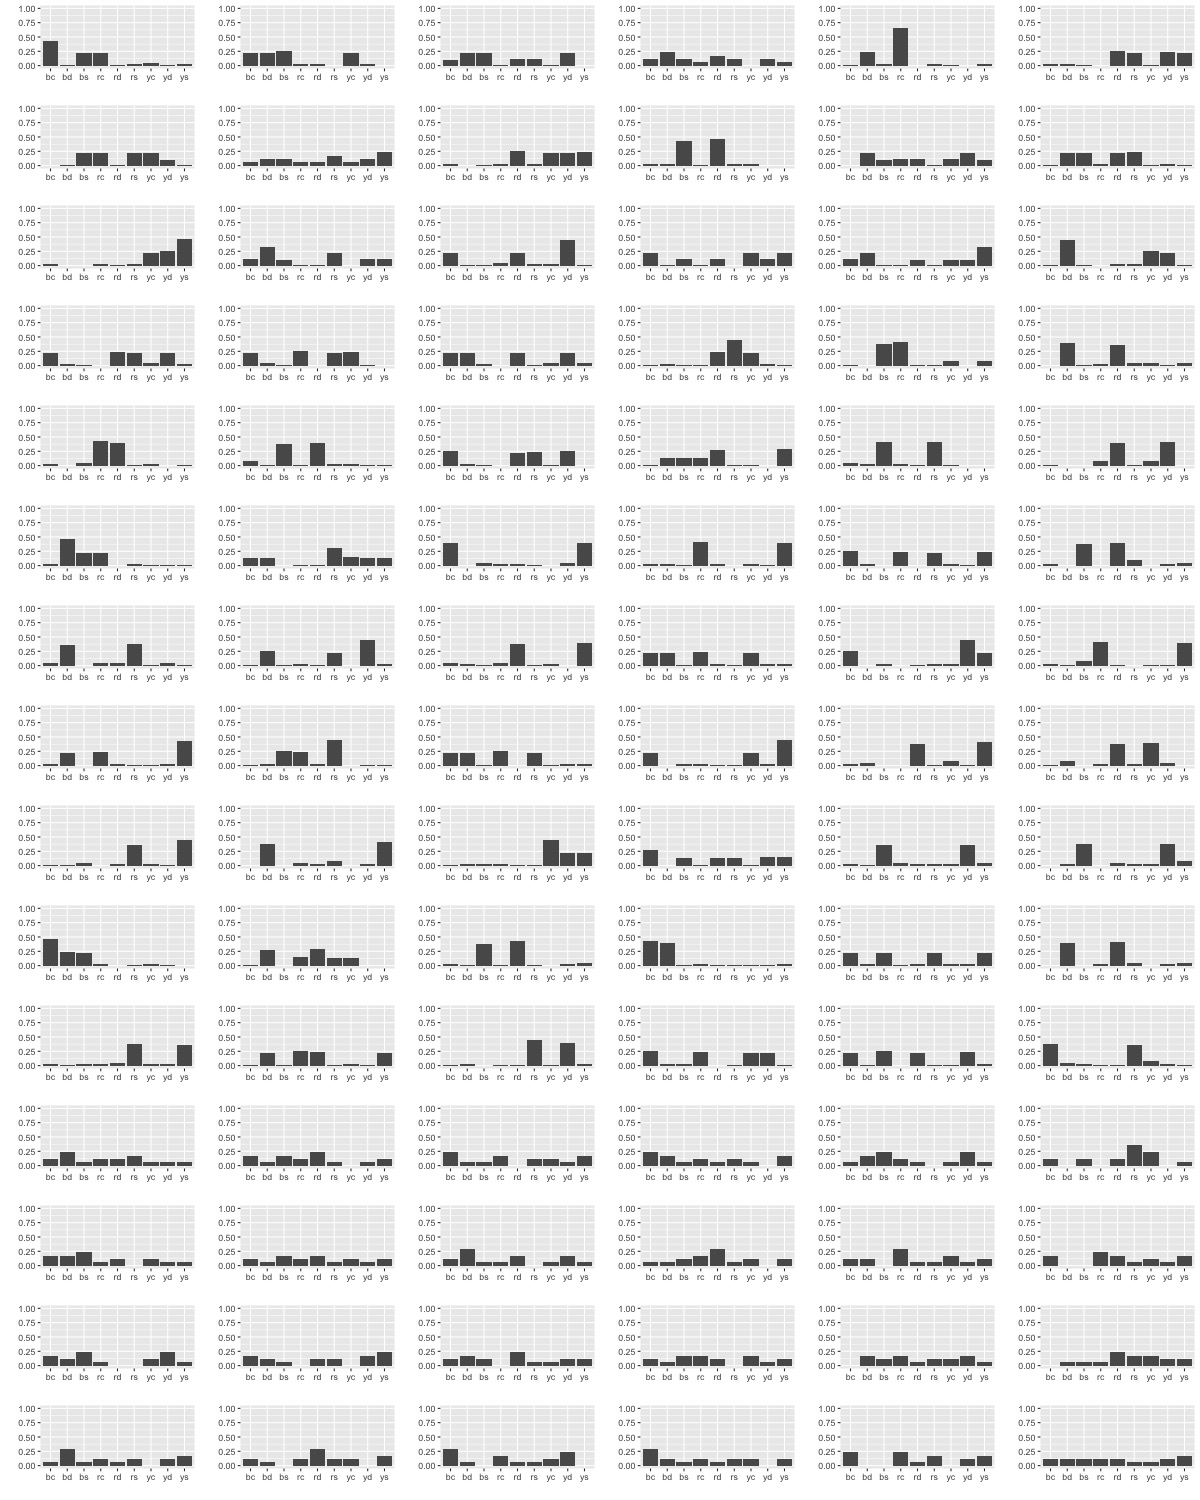
\includegraphics[width=.8\linewidth]{sim_trials}
  \caption{Simulation raw selections summary. Each row is for one trial, and each column is for one task. For each sub-figure, y-axis is percentage, and x-axis from left to right is: bc, bd, bs, rc, rd, rs, yc, yd, ys.}
  \label{fig:sim_raw}
\end{figure}

\begin{figure}[h!]
  \centering
  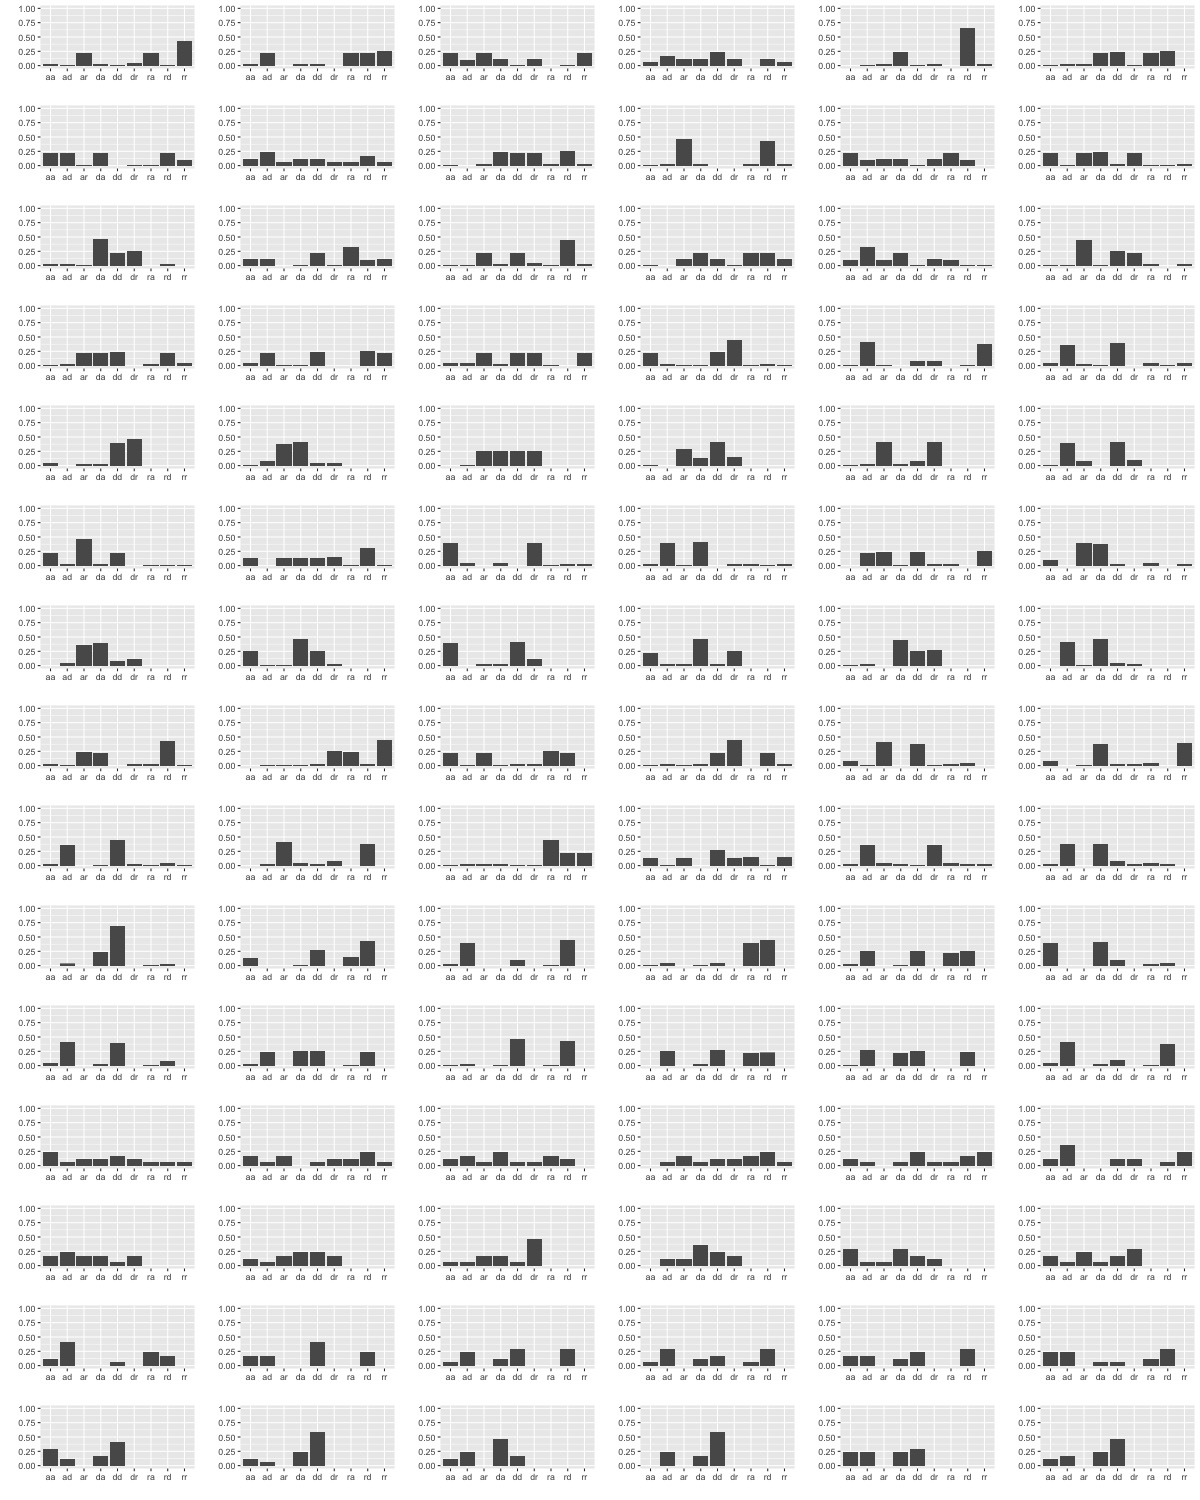
\includegraphics[width=.8\linewidth]{sim_trials_relative}
  \caption{Relative selections summary. Each row is for one trial, and each column is for one task. For each sub-figure, y-axis is percentage, and x-axis from left to right is: aa, ad, ar, da, dd, dr, ra, rd, rr.}
\end{figure}

% Aggregated by groups
\clearpage

\subsection{Aggregated by relative selections}

The normative model does not show specific patterns towards each learning task (Figure~\ref{fig:sim_agg_groups}). It does show a tendency to concentrate on one selection as the generalization scenarios further differs from the learning scenarios (last figure in Figure~\ref{fig:sim_agg_trials}), but it predicts a different concentration point compared with participant data.

\begin{figure}[h!]
  \centering
  \begin{subfigure}[t]{0.25\textwidth}
    \centering
    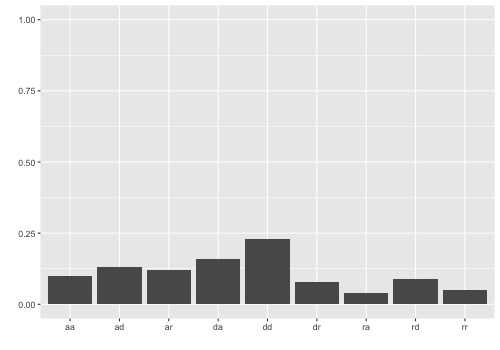
\includegraphics[width=\linewidth]{sim_agg_g1} 
    \caption{To the same shape} \label{fig:sim_agg_g1}
  \end{subfigure}
  \begin{subfigure}[t]{0.25\textwidth}
    \centering
    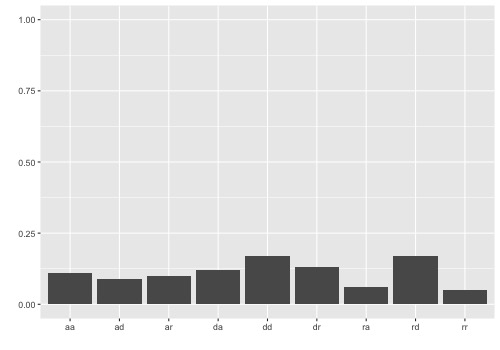
\includegraphics[width=\linewidth]{sim_agg_g3} 
    \caption{To the same color} \label{fig:sim_agg_g3}
  \end{subfigure}
  \begin{subfigure}[t]{0.25\textwidth}
    \centering
    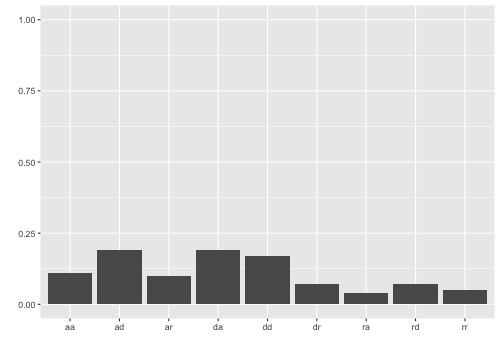
\includegraphics[width=\linewidth]{sim_agg_g6} 
    \caption{To the same object} \label{fig:sim_agg_g6}
  \end{subfigure}

  \vspace{1em}
  \begin{subfigure}[t]{0.25\textwidth}
    \centering
    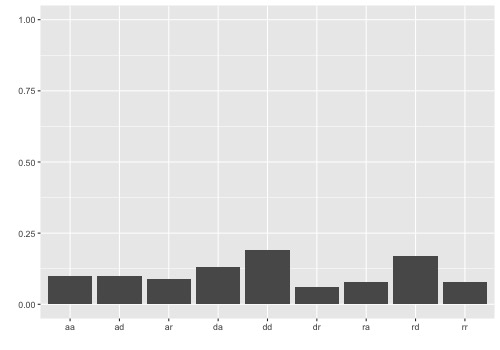
\includegraphics[width=\linewidth]{sim_agg_g2} 
    \caption{To a different shape} \label{fig:sim_agg_g2}
  \end{subfigure}
  \begin{subfigure}[t]{0.25\textwidth}
    \centering
    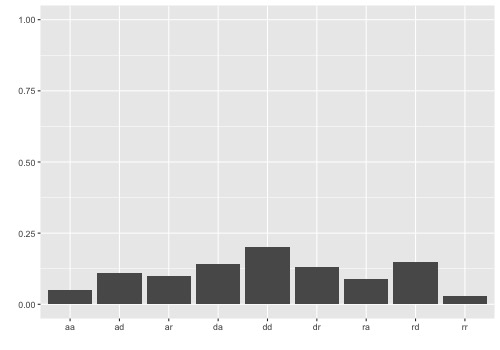
\includegraphics[width=\linewidth]{sim_agg_g4} 
    \caption{To a different color} \label{fig:sim_agg_g4}
  \end{subfigure}
  \begin{subfigure}[t]{0.25\textwidth}
    \centering
    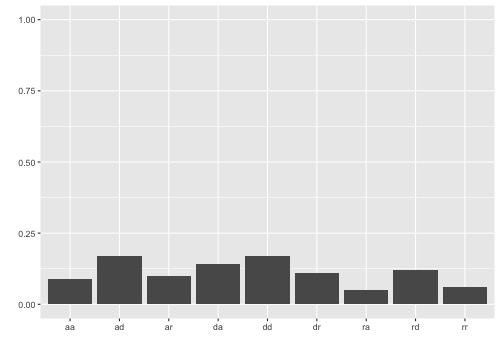
\includegraphics[width=\linewidth]{sim_agg_g5} 
    \caption{To a different object} \label{fig:sim_agg_g5}
  \end{subfigure}
  \caption{Aggregated relative selections per task. For each sub-figure, y-axis is percentage, and x-axis from left to right is: aa, ad, ar, da, dd, dr, ra, rd, rr.}
  \label{fig:sim_agg_groups}
\end{figure}

% Aggregated by trials
\begin{figure}[h!]
  \centering
  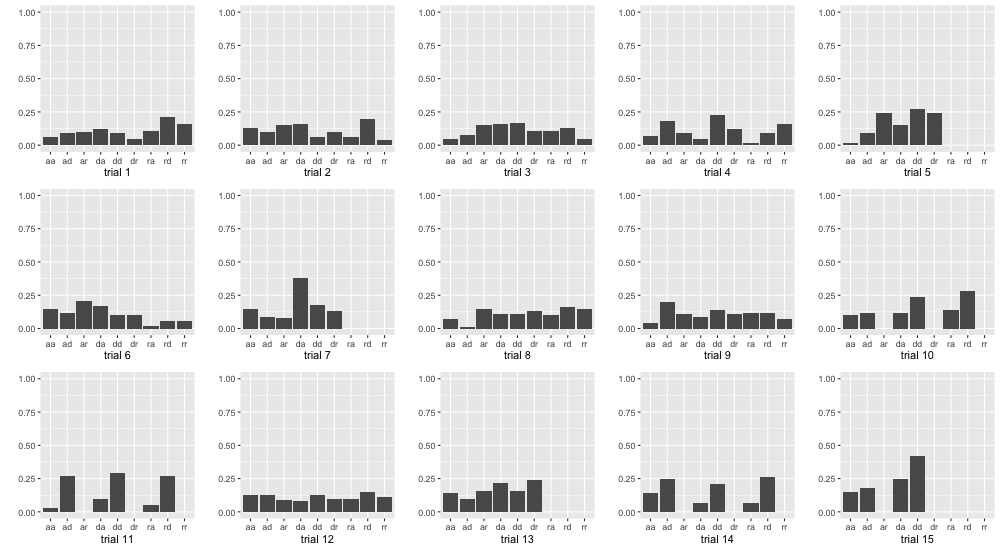
\includegraphics[width=.8\linewidth]{sim_agg_trials}
  \caption{Aggregated relative selections per trial. For each sub-figure, y-axis is percentage, and x-axis from left to right is: aa, ad, ar, da, dd, dr, ra, rd, rr.}
  \label{fig:sim_agg_trials}
\end{figure}

\section{Compliance with theories}

\begin{itemize}
\item learn01: to the same shape as magic stone (and kept color unchanged)
\item learn02: to a different shape as magic stone (and kept color unchanged)
\item learn03: to the same color as magic stone (and kept shape unchanged)
\item learn04: to a different color as magic stone (and kept shape unchanged)
\item learn05: To a different object
\item learn06: To the same object as the magic stone
\end{itemize}

\subsection{Total compliance}
\begin{figure}[h!]
  \centering
  \begin{subfigure}[t]{0.4\textwidth}
    \centering
    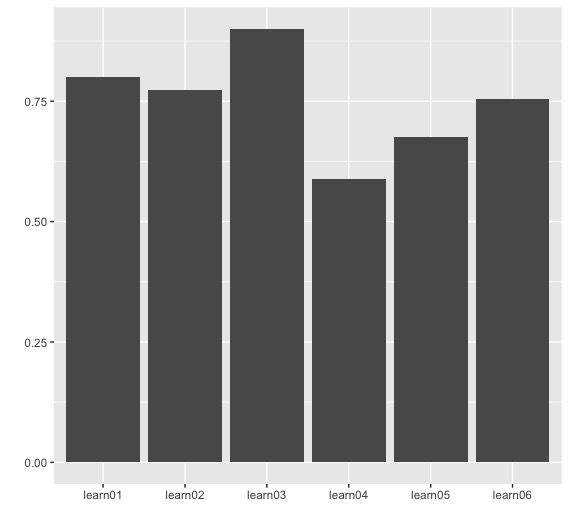
\includegraphics[width=\linewidth]{total_compliance_per_learning_condition} 
    \caption{Per learning condition}
  \end{subfigure}
  \hfill
  \begin{subfigure}[t]{0.55\textwidth}
    \centering
    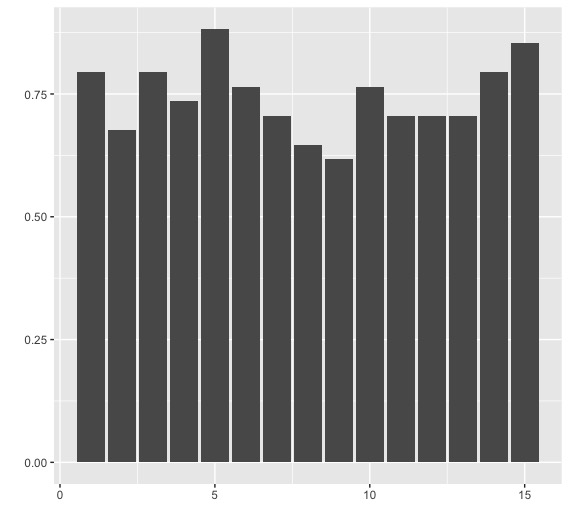
\includegraphics[width=\linewidth]{total_compliance_per_trial} 
    \caption{Per generalization trial}
  \end{subfigure}
  \caption{Percent of selections that comply with the underlying theory, aggregated per learning condition and per generalization trial separately.}
  \label{fig:total_comp}
\end{figure}

\newpage
\subsection{Details}

For learn01 - learn04, take the description outside of the parenthesis as `r1', and description inside the parenthesis as `r2', we can compare to what extent participants comply with such theories.

\begin{figure}[h!]
  \centering
  \begin{subfigure}[t]{0.3\textwidth}
    \centering
    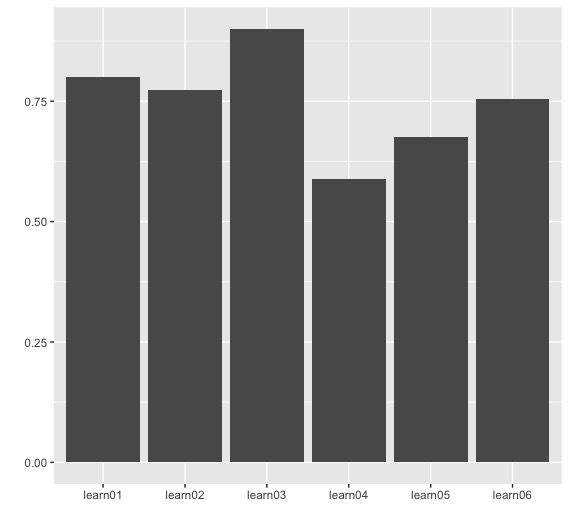
\includegraphics[width=\linewidth]{total_compliance_per_learning_condition} 
    \caption{Overall compliance}
  \end{subfigure}
  \hfill
  \begin{subfigure}[t]{0.6\textwidth}
    \centering
    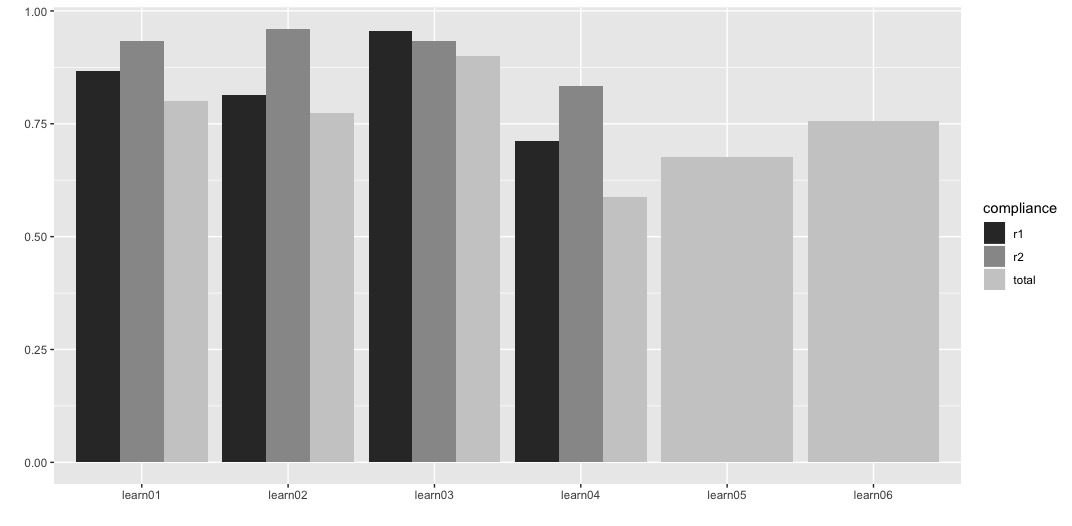
\includegraphics[width=\linewidth]{compliance_per_learning_condition} 
    \caption{Split by sub-rule compliance}
  \end{subfigure}
  \caption{Percent of selections that comply with the underlying theory, aggregated per learning condition.}
  \label{fig:comp_learn}
\end{figure}

\begin{figure}[h!]
  \centering
  \begin{subfigure}[t]{0.35\textwidth}
    \centering
    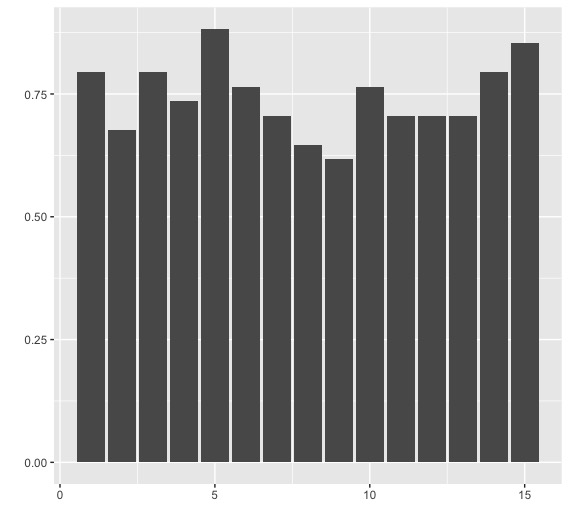
\includegraphics[width=\linewidth]{total_compliance_per_trial} 
    \caption{Overall compliance}
  \end{subfigure}
  \hfill
  \begin{subfigure}[t]{0.6\textwidth}
    \centering
    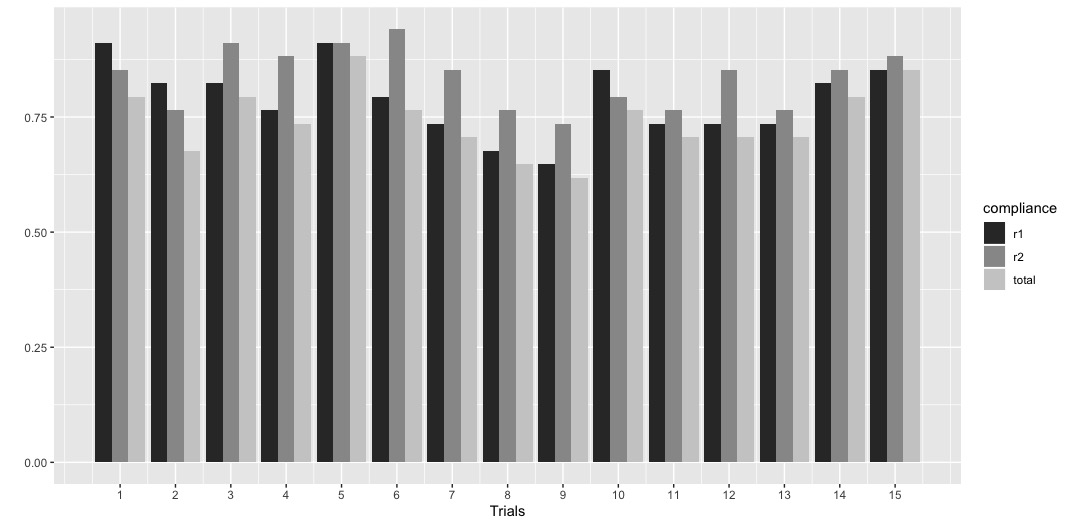
\includegraphics[width=\linewidth]{compliance_per_trial} 
    \caption{Split by sub-rule compliance}
  \end{subfigure}
  \caption{Percent of selections that comply with the underlying theory, aggregated per generalization trial.}
  \label{fig:comp_trial}
\end{figure}

\newpage
\subsection{Individual}
\begin{figure}[h!]
  \centering
  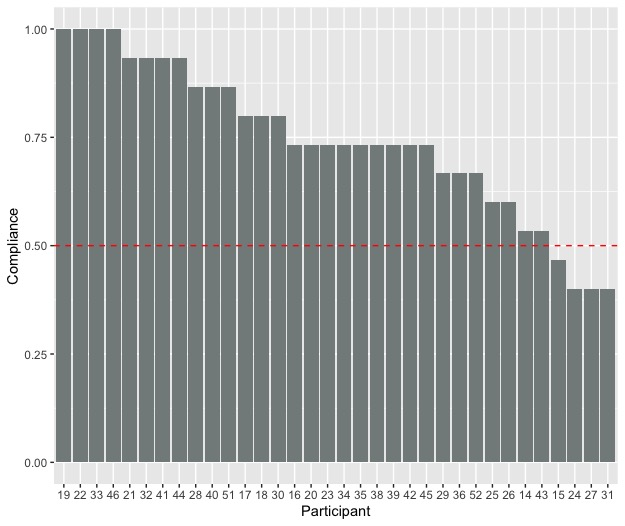
\includegraphics[width=.8\linewidth]{individual_compliance} 
  \caption{Compliance per participant.} 
  \label{fig:comp_ppt}
\end{figure}


\section{Homogeneity}

To measure how participant selections vary across learning conditions, define trial $i$'s variation $v_i := (U - 1) /n $ where $U$ is the number of unique selections from all participants for trial $i$, and $n$ is the number of participants in this trial. 
We take $U - 1$ because of the intuition that if all participants select the same stone, the number of unique selections is 1 and variation is 0.
Variation $V_J$ for a learning condition $J$ is therefore defined as $V_j := \sum_{i \in J}v_i$, for all generalization trial $i$ under learning condition $J$.

Variations for the six above mentioned learning conditions are as follows

\begin{table}[b]
\centering
\begin{tabular}{l|l|l}
Learning condition & Theory & Variation \\
\hline
1                  & To the same shape & 2.75 \\
2                  & To a different shape & 3.00 \\
3                  & To the same color & 1.33  \\
4                  & To a different color & 5.16  \\
5                  & To a different object & 4.57  \\
6                  & To the same object & 3.00  \\
\end{tabular}
\end{table}




\end{document}